\documentclass[tikz,border=0.12in]{standalone}
\usepackage{tikz}
\usepackage{amssymb}
\usetikzlibrary{positioning, arrows.meta, fit, backgrounds, calc}
\usepackage[T1]{fontenc}
\usepackage[scaled=0.95]{helvet}
\renewcommand{\familydefault}{\sfdefault}
\hyphenpenalty=10000\exhyphenpenalty=10000  % no mid-word hyphenation

% ---- Miami University official brand palette ----
\definecolor{miamired}{HTML}{C41230}    % curated corpus (the core)
\definecolor{slate}{HTML}{3E5468}       % source documents
\definecolor{cornyellow}{HTML}{EFDB72}  % downstream use
\definecolor{okgreen}{HTML}{2E7D5B}     % completed-metric checkmark

\newcommand{\sep}{\,\textcolor{black!35}{\textbar}\,}   % source-list separator
\newcommand{\tk}[1]{\underline{\textbf{#1}}}            % task label: bold + underline

\tikzset{
  srccard/.style   = {rectangle, rounded corners, draw=slate, thick, fill=slate!5,
                      align=left, text width=5.0cm, inner sep=7pt, font=\small, minimum height=1.8cm},
  corpusframe/.style = {rectangle, rounded corners=8pt, draw=miamired, ultra thick, fill=miamired!5,
                      align=left, text width=5.2cm, inner sep=10pt, font=\small, minimum height=8.4cm},
  dswide/.style    = {rectangle, rounded corners, draw=cornyellow!62!black, thick, fill=cornyellow!25,
                      align=center, text width=4.4cm, inner sep=7pt, font=\small, text=black!88,
                      minimum height=1.5cm},
  dsnarrow/.style  = {rectangle, rounded corners, draw=cornyellow!62!black, thick, fill=cornyellow!25,
                      align=center, text width=2.7cm, inner sep=6pt, font=\small, text=black!88,
                      minimum height=2.7cm},
  stagehead/.style = {font=\large\bfseries, text=black!85, align=center},
  feed/.style      = {very thick, -{Stealth[length=3mm]}, draw=slate!70},
  flow/.style      = {ultra thick, -{Stealth[length=3.2mm]}, draw=miamired!70},
}
\newcommand{\stagerule}[1]{{\color{miamired}\rule{#1}{1.1pt}}}

\begin{document}
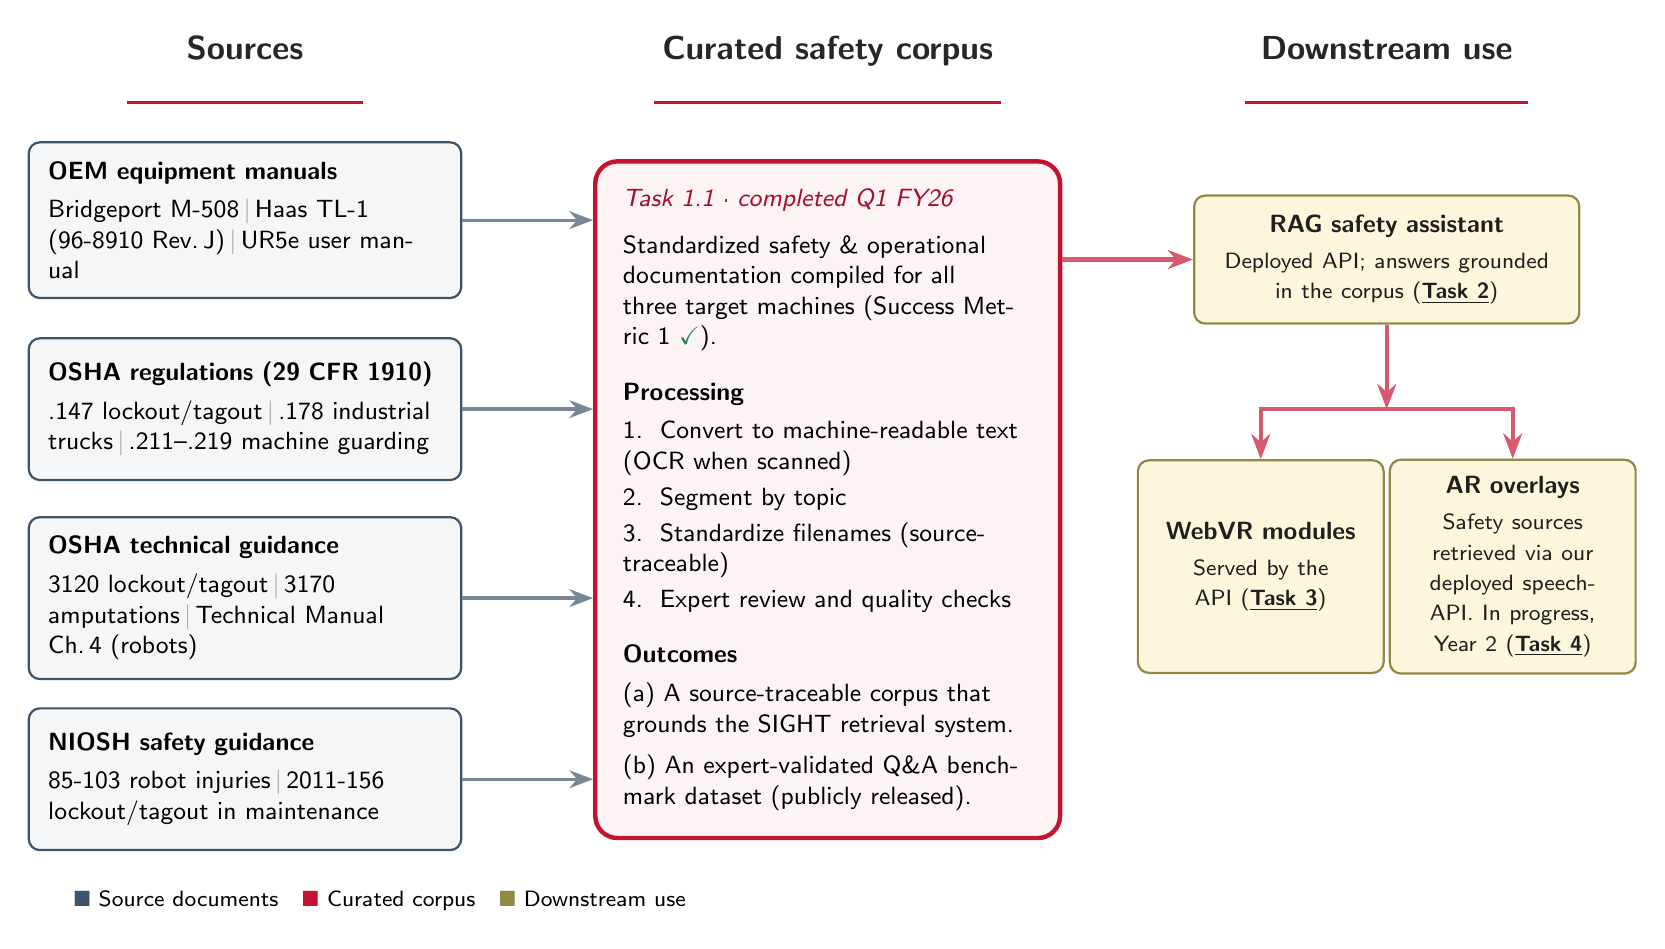
\begin{tikzpicture}

% =============== STAGE HEADERS ===============
\node[stagehead] at (0,10.0)    {Sources\\[2pt]\stagerule{3.0cm}};
\node[stagehead] at (7.4,10.0)  {Curated safety corpus\\[2pt]\stagerule{4.4cm}};
\node[stagehead] at (14.5,10.0) {Downstream use\\[2pt]\stagerule{3.6cm}};

% =============== STAGE 1: SOURCE DOCUMENTS ===============
\node (s1) [srccard] at (0,8.1) {\textbf{OEM equipment manuals}\\[3pt]%
  Bridgeport M-508\sep Haas TL-1 \mbox{(96-8910 Rev.\,J)}\sep UR5e user manual};
\node (s2) [srccard] at (0,5.7) {\textbf{OSHA regulations (29 CFR 1910)}\\[3pt]%
  .147 lockout/tagout\sep .178 industrial trucks\sep .211--.219 machine guarding};
\node (s3) [srccard] at (0,3.3) {\textbf{OSHA technical guidance}\\[3pt]%
  3120 \mbox{lockout/tagout}\sep 3170 \mbox{amputations}\sep Technical Manual Ch.\,4 (robots)};
\node (s4) [srccard] at (0,1.0) {\textbf{NIOSH safety guidance}\\[3pt]%
  85-103 robot injuries\sep 2011-156 \mbox{lockout/tagout} in maintenance};

% =============== STAGE 2: CURATED CORPUS ===============
\node (corpus) [corpusframe] at (7.4,4.55) {%
  {\color{miamired!85!black}\itshape Task~1.1 \textperiodcentered\ completed Q1 FY26}\\[6pt]
  Standardized safety \& operational documentation compiled for all three target machines (Success Metric~1~{\color{okgreen}\checkmark}).\\[9pt]
  {\bfseries Processing}\\[3pt]
  1.~~Convert to machine-readable text (OCR when scanned)\\[2pt]
  2.~~Segment by topic\\[2pt]
  3.~~Standardize filenames (source-traceable)\\[2pt]
  4.~~Expert review and quality checks\\[9pt]
  {\bfseries Outcomes}\\[3pt]
  (a)~A source-traceable corpus that grounds the SIGHT retrieval \mbox{system}.\\[4pt]
  (b)~An expert-validated Q\&A benchmark dataset (publicly released).};

% source -> corpus feeds
\foreach \s in {s1,s2,s3,s4}
  \draw[feed] (\s.east) -- (corpus.west |- \s.east);

% =============== STAGE 3: DOWNSTREAM USE ===============
\node (rag) [dswide]   at (14.5,7.6) {\textbf{RAG safety assistant}\\[2pt]%
  {\footnotesize Deployed API; answers grounded in the corpus (\tk{Task~2})}};
\node (vr)  [dsnarrow] at (12.9,3.7) {\textbf{WebVR modules}\\[2pt]%
  {\footnotesize Served by the API (\tk{Task~3})}};
\node (ar)  [dsnarrow] at (16.1,3.7) {\textbf{AR overlays}\\[2pt]%
  {\footnotesize Safety sources retrieved via our deployed speech-API. In progress, Year~2 (\tk{Task~4})}};

% corpus -> RAG, then a clean forked arrow RAG -> {VR, AR}
\draw[flow] (corpus.east |- rag.west) -- (rag.west);
\coordinate (fork) at (14.5,5.7);
\draw[flow] (rag.south) -- (fork);
\draw[flow] (fork) -| (vr.north);
\draw[flow] (fork) -| (ar.north);

% =============== LEGEND ===============
\node[font=\footnotesize, anchor=west] at (-2.3,-0.55) {%
  \textcolor{slate}{$\blacksquare$}~Source documents\quad
  \textcolor{miamired}{$\blacksquare$}~Curated corpus\quad
  \textcolor{cornyellow!62!black}{$\blacksquare$}~Downstream use};

\end{tikzpicture}
\end{document}
